
% Styl dwustronny z domyślną wielkością czcionki 10pt oraz oddzieloną stroną tytułową (titlepage).
% Domyślnie rodziały rozpoczynają się na stronie prawej (openright).
\documentclass{book}



% Pakiet babel dla polskiego języka powoduje konflikt z pakietem amssymb.
% Polecenie '\lll' definiują oba pakiety - porządana jest druga definicja.
\let\lll\undefined


% Kodowanie dokumentu
\usepackage[utf8]{inputenc}

% Dowolny rozmiar czcionek, kodowanie znaków
\usepackage{lmodern}

% Polskie wcięcia akapitów
\usepackage{indentfirst}

% Polskie łamanie wyrazów
\usepackage[plmath]{polski}

% Przecinek w wyrażeniach matematycznych zamiast kropki
\usepackage{icomma}

% Polskie formatowanie typograficzne
\frenchspacing

% Zapewnia liczne usprawnienia wyświetlania i organizacji matematycznych formuł. 
\usepackage{amsmath}

% Wprowadza rozszerzony zestaw symboli m.in. \leadsto
\usepackage{amssymb}

% Dodatkowa, ,,kręcona'' czcionka matematyczna
\usepackage{mathrsfs}

% Dodatkowe wsparcie dla środowiska mathbb, które nie wspiera domyślnie cyfr (\mathbb{})
\usepackage{bbold}

% Fixes/improves amsmath
\usepackage{mathtools}


% ***************************************************************************************************
% Kolory  
% ***************************************************************************************************

% Umożliwia kolorowanie poszczególnych komórek tabeli
\usepackage[table]{xcolor}% http://ctan.org/pkg/

% Umożliwia łatwą zmianę koloru linii w tabeli
\usepackage{tabu}

% Umożliwia rozszerzoną kontrolę nad kolorami.
\usepackage{xcolor}

% Definicje kolorów
\definecolor{lgray}{HTML}{9F9F9F}
\definecolor{dgray}{HTML}{5F5F5F}
% lgray				-	nazwa nowo zdefiniowanego koloru
% HTML				-	model kolorów
% CCCCCC			-	wartość koloru zgodna z modelem

% ***************************************************************************************************
% Algorytmy 
% ***************************************************************************************************

% Udostępnia środowisko do konstruowania pseudokodów
\usepackage[ruled,vlined,linesnumbered,longend,algochapter]{algorithm2e}
% ruled	- poziome kreski na początku i końcu algorytmu, podpis na górze oddzielony również kreską poziomą
% vlined - pionowe kreski łączące początek polecenia z jego końcem
% linesnumbered	- numerowanie kolejnych wierszy algorytmu
% longend - długie końcówki np. ifend, forend itd.
% algochapter - numeracja z rozdziałami

% Zamiana nazwy środowiska z domyślnej "Algorithm X" na "Pseudokod X"
\newenvironment{pseudokod}[1][htb]{
	\renewcommand{\algorithmcfname}{Pseudokod}
	\begin{algorithm}[#1]%
	}{
\end{algorithm}
}

% Zmiana rozmiaru komentarzy
\newcommand\algcomment[1]{
	\footnotesize{#1}
}

% Ustawienie zadanego stylu dla komentarzy
\SetCommentSty{algcomment}

% Wyśrodkowana tylda
\usepackage{textcomp}%
\newcommand{\textapprox}{\raisebox{0.5ex}{\texttildelow}}

% Listowanie kodów źródłowych
\usepackage{listings} 
\renewcommand{\lstlistingname}{Kod źródłowy} % Polska nazwa listingu

% Definicjes pecjalnych znaków, które nie są obsługiwane w środowisku listing
\lstset{literate=
	{ż}{{\.{z}}}1	{ź}{{\'{z}}}1
	{ć}{{\'{c}}}1		{ń}{{\'{n}}}1
	{ą}{{\c a}}1		{ś}{{\'{s}}}1
	{ł}{{\l}}1		{ę}{{\c{e}}}1
	{ó}{{\'{o}}}1	{á}{{\'a}}1
	{é}{{\'e}}1		{í}{{\'i}}1
	{ó}{{\'o}}1		{ú}{{\'u}}1
	{ù}{{\`u}}1		{Á}{{\'A}}1
	{É}{{\'E}}1		{Í}{{\'I}}1
	{Ó}{{\'O}}1		{Ú}{{\'U}}1
	{à}{{\`a}}1		{è}{{\'e}}1
	{ì}{{\`i}}1		{ò}{{\`o}}1
	{ò}{{\`o}}1		{À}{{\`A}}1
	{È}{{\'E}}1		{Ì}{{\`I}}1
	{Ò}{{\`O}}1		{Ò}{{\`O}}1
	{ä}{{\"a}}1		{ë}{{\"e}}1
	{ï}{{\"i}}1		{ö}{{\"o}}1
	{ü}{{\"u}}1		{Ä}{{\"A}}1
	{Ë}{{\"E}}1		{Ï}{{\"I}}1
	{Ö}{{\"O}}1		{Ü}{{\"U}}1
	{â}{{\^a}}1		{ê}{{\^e}}1
	{î}{{\^i}}1		{ô}{{\^o}}1
	{û}{{\^u}}1		{Â}{{\^A}}1
	{Ê}{{\^E}}1		{Î}{{\^I}}1
	{Ô}{{\^O}}1	{Û}{{\^U}}1
	{œ}{{\oe}}1		{Œ}{{\OE}}1
	{æ}{{\ae}}1		{Æ}{{\AE}}1
	{ß}{{\ss}}1		{ç}{{\c c}}1
	{Ç}{{\c C}}1		{ø}{{\o}}1
	{å}{{\r a}}1		{Å}{{\r A}}1
	{€}{{\EUR}}1	{£}{{\pounds}}1
}

% ***************************************************************************************************
% Marginesy 
% ***************************************************************************************************

% Ustawienia rozmiarów stron i ich marginesów
\usepackage[headheight=18pt, top=25mm, bottom=25mm, left=25mm, right=25mm]{geometry}
% headheight		-	wysokość tytułów
% top				-	margines górny
% bottom			-	margines dolny
% left				-	margines lewy
% right				-	margines prawy

% Usunięcie górnego marginesu dla środowisk
\makeatletter
\setlength\@fptop{0\p@}	
\makeatother

% ***************************************************************************************************
% Styl 
% ***************************************************************************************************

% Definiuje środowisko 'titlingpage', które zapewnia pełną kontrolę nad układem strony tytułowej.
\usepackage{titling}


% Umożliwia modyfikowanie stylu spisu treści
\usepackage{tocloft}	

\tocloftpagestyle{tableOfContentStyle}

% Definiowanie własnych stylów nagłówków i/lub stopek
\usepackage{fancyhdr}

% Domyślny styl dla pracy 
\fancypagestyle{custom}{
	\fancyhf{}									% wyczyść stopki i nagłówki
	\fancyhead[RO]{								% Prawy, nieparzysty nagłówek
		\hrulefill \hspace{16pt} \large Rozdział \thechapter
		\put(-472.1, 12.1){%
			\makebox(0,0)[l]{%
				
\includegraphics[width=0.05\textwidth]{pwr-logo}
			}
		}
		\put(-443,5.5){%
			\makebox(0,0)[l]{%
				\small Politechnika Wrocławska
			}
		}
	}
	\fancyhead[LE]{								% Lewy, parzysty nagłówek
		\large Rozdział \thechapter \hspace{16pt} \hrulefill 
		\put(-22, 12.1){%
			\makebox(0,0)[l]{%
				
\includegraphics[width=0.05\textwidth]{wppt-logo}
			}
		}
		\put(-210,5.5){%
			\makebox(0,0)[l]{%
				\small Wydział Podstawowych Problemów Techniki
			}
		}
	}
	\fancyfoot[LE,RO]{							
		\thepage
	}
	\renewcommand{\headrulewidth}{0pt}		
	\renewcommand{\footrulewidth}{0.2pt}	
	
}


% Domyślny styl dla bibliografii
\fancypagestyle{bibliographyStyle}{
	\fancyhf{}									% wyczyść stopki i nagłówki
	\fancyhead[RO]{								% Prawy, nieparzysty nagłówek
		\hrulefill \hspace{16pt} \large Dodatek \thechapter
		\put(-472.1, 12.1){%
			\makebox(0,0)[l]{%
				
\includegraphics[width=0.05\textwidth]{pwr-logo}
			}
		}
		\put(-443,5.5){%
			\makebox(0,0)[l]{%
				\small Politechnika Wrocławska
			}
		}
	}
	\fancyhead[LE]{								% Lewy, parzysty nagłówek
		\large Bibliografia \hspace{16pt} \hrulefill 
		\put(-22, 12.1){%
			\makebox(0,0)[l]{%
				
\includegraphics[width=0.05\textwidth]{wppt-logo}
			}
		}
		\put(-210,5.5){%
			\makebox(0,0)[l]{%
				\small Wydział Podstawowych Problemów Techniki
			}
		}
	}
	\fancyfoot[LE,RO]{							% Stopki
		\thepage
	}
	\renewcommand{\headrulewidth}{0pt}			% Grubość linii w nagłówku
	\renewcommand{\footrulewidth}{0.2pt}		% Grubość linii w stopce
}

% Domyślny styl dla dodatków
\fancypagestyle{appendixStyle}{
	\fancyhf{}									% wyczyść stopki i nagłówki
	\fancyhead[RO]{								% Prawy, nieparzysty nagłówek
		\hrulefill \hspace{16pt} \large Dodatek \thechapter
		\put(-472.1, 12.1){%
			\makebox(0,0)[l]{%
				
\includegraphics[width=0.05\textwidth]{pwr-logo}
			}
		}
		\put(-443,5.5){%
			\makebox(0,0)[l]{%
				\small Politechnika Wrocławska
			}
		}
	}
	\fancyhead[LE]{								% Lewy, parzysty nagłówek
		\large Dodatek \thechapter \hspace{16pt} \hrulefill 
		\put(-22, 12.1){%
			\makebox(0,0)[l]{%
				
\includegraphics[width=0.05\textwidth]{wppt-logo}
			}
		}
		\put(-210,5.5){%
			\makebox(0,0)[l]{%
				\small Wydział Podstawowych Problemów Techniki
			}
		}
	}
	\fancyfoot[LE,RO]{							% Stopki
		\thepage
	}
	\renewcommand{\headrulewidth}{0pt}			% Grubość linii w nagłówku
	\renewcommand{\footrulewidth}{0.2pt}		% Grubość linii w stopce
}

% Osobny styl dla stron zaczynających rozdział/spis treści itd. (domyślnie formatowane jako "plain")
\fancypagestyle{chapterBeginStyle}{
	\fancyhf{}%
	\fancyfoot[LE,RO]{
		\thepage
	}
	\renewcommand{\headrulewidth}{0pt}
	\renewcommand{\footrulewidth}{0.2pt}
}

% Styl dla pozostałych stron spisu treści
\fancypagestyle{tableOfContentStyle}{
	\fancyhf{}%
	\fancyfoot[LE,RO]{
		\thepage
	}
	\renewcommand{\headrulewidth}{0pt}
	\renewcommand{\footrulewidth}{0.2pt}
}

% Formatowanie tytułów rozdziałów i/lub sekcji
\usepackage{titlesec}

% Formatowanie tytułów rozdziałów
\titleformat{\chapter}[hang]					% kształt
{
	\vspace{-15ex}
	\Huge
	\bfseries
}												% formatowanie tekstu modyfikowanego elementu
{}												% etykieta występująca przed tekstem modyfikowanego elementu, niewidoczna w spisie treści
{
	10pt
}												% odstęp formatowanego tytułu od lewego marginesu/etykiety
{
	\Huge
	\bfseries
}												% formatowanie elementów przed modyfikowanym tytułem
[
\vspace{0ex}
%\rule{\textwidth}{0.4pt}
%\vspace{-4ex}
]												% dodatkowe formatowanie stosowane poniżej modyfikowanego tytułu


% Formatowanie tytułów sekcji
\titleformat{\section}[hang]					% kształt
{
	\vspace{1ex}
%	\titlerule\vspace{1ex}
	\Large\bfseries
}												% formatowanie tekstu modyfikowanego elementu
{
	\thesection									% etykieta występująca przed tekstem modyfikowanego elementu, niewidoczna w spisie treści
}
{
	0pt
}												% odstęp formatowanego tytułu od lewego marginesu/etykiety
{
	\Large
	\bfseries
}												% formatowanie elementów przed modyfikowanym tytułem

% ***************************************************************************************************
% Linki
% ***************************************************************************************************

% Umożliwia wstawianie hiperłączy do dokumentu
\usepackage{hyperref}							% Aktywuje linki

\hypersetup{
	colorlinks	=	true,					% Koloruje tekst zamiast tworzyć ramki.
	linkcolor		=	blue,					% Kolory: referencji,
        citecolor		=	blue,					% cytowań,
	urlcolor		=	blue					% hiperlinków.
}

% Do stworzenia hiperłączy zostanie użyta ta sama (same) czcionka co dla reszty dokumentu
\urlstyle{same}


\setlength{\tabcolsep}{18pt}
\renewcommand{\arraystretch}{1.5}


% ***************************************************************************************************
% Linki
% ***************************************************************************************************

% Umożliwia zdefiniowanie własnego stylu wyliczeniowego
\usepackage{enumitem}

% Nowa lista numerowana z trzema poziomami
\newlist{myitemize}{itemize}{3}

% Definicja wyglądu znacznika pierwszego poziomu
\setlist[myitemize,1]{
	label		=	\textbullet,
	leftmargin	=	4mm}

% Definicja wyglądu znacznika drugiego poziomu
\setlist[myitemize,2]{
	label		=	$\diamond$,
	leftmargin	=	8mm}

% Definicja wyglądu znacznika trzeciego poziomu
\setlist[myitemize,3]{
	label		=	$\diamond$,
	leftmargin	=	12mm
}

% ***************************************************************************************************
% Inne pakiety
% ***************************************************************************************************

% Dołączanie rysunków
\usepackage{graphicx}

% Figury i przypisy
\usepackage{caption}
\usepackage{subcaption}

% Umożliwia tworzenie przypisów wewnątrz środowisk
\usepackage{footnote}

% Umożliwia tworzenie struktur katalogów
\usepackage{dirtree}

% Rozciąganie komórek tabeli na wiele wierszy
\usepackage{multirow}

% Precyzyjne obliczenia szerokości/wysokości dowolnego fragmentu wygenerowanego przez LaTeX
\usepackage{calc}

% ***************************************************************************************************
% Matematyczne skróty
% ***************************************************************************************************

% Skrócony symbol liczb rzeczywistych
\newcommand{\RR}{\mathbb{R}}

% Skrócony symbol liczb naturalnych
\newcommand{\NN}{\mathbb{N}}

% Skrócony symbol liczb wymiernych
\newcommand{\QQ}{\mathbb{Q}}

% Skrócony symbol liczb całkowitych
\newcommand{\ZZ}{\mathbb{Z}}

% Skrócony symbol logicznej implikacji
\newcommand{\IMP}{\rightarrow}

% Skrócony symbol  logicznej równoważności
\newcommand{\IFF}{\leftrightarrow}

% ***************************************************************************************************
% Środowiska
% ***************************************************************************************************

% Środowisko do twierdzeń
\newtheorem{theorem}{Twierdzenie}[chapter]

% Środowisko do lematów
\newtheorem{lemma}{Lemat}[chapter]

% Środowisko do przykładów
\newtheorem{example}{Przykład}[chapter]

% Środowisko do wniosków
\newtheorem{corollary}{Wniosek}[chapter]

% Środowisko do definicji
\newtheorem{definition}{Definicja}[chapter]

% Środowisko do dowodów
\newenvironment{proof}{
	\par\noindent \textbf{Dowód.}
}{
\begin{flushright}
	\vspace*{-6mm}\mbox{$\blacklozenge$}
\end{flushright}
}

% Środowisko do uwag
\newenvironment{remark}{
	\bigskip \par\noindent \small \textbf{Uwaga.}
}{
\begin{small}
	\vspace*{4mm}
\end{small}
}


\hyphenation{wszy-stkich ko-lu-mnę każ-da od-leg-łość
	dzie-dzi-ny dzie-dzi-na rów-nych rów-ny
	pole-ga zmie-nna pa-ra-met-rów wzo-rem po-cho-dzi
	o-trzy-ma wte-dy wa-run-ko-wych lo-gicz-nie
	skreś-la-na skreś-la-ną cał-ko-wi-tych wzo-rów po-rzą-dek po-rząd-kiem
	przy-kład pod-zbio-rów po-mię-dzy re-pre-zen-to-wa-ne
	rów-no-waż-ne bi-blio-te-kach wy-pro-wa-dza ma-te-ria-łów
	prze-ka-za-nym skoń-czo-nym moż-esz na-tu-ral-na cią-gu tab-li-cy
	prze-ka-za-nej od-po-wied-nio}

\def\blankpage{%
	\clearpage%
	\thispagestyle{empty}%
	\addtocounter{page}{-1}%
	\null%
	\clearpage}

\frontmatter
	\renewcommand{\lstlistlistingname}{Spis kodów źródłowych}
	
\begin{document}

	\begin{titlingpage}
	\vspace*{\fill}
	\begin{center}
		\begin{picture}(300,510)
			\put(11,520){\makebox(0,0)[l]{\large \textsc{Wydział Podstawowych Problemów Techniki}}}
			\put(11,500){\makebox(0,0)[l]{\large \textsc{Politechnika Wrocławska}}}
			\put(70,320){\Huge \textsc{Aplikacja wspomagająca}}
			\put(70,280){\Huge \textsc{zarządzanie zadaniami}}

			\put(90,200){\makebox(0,0)[l]{\large \textsc{Daniel Drapała}}}
			\put(90,180){\makebox(0,0)[l]{\large \textsc{Nr indeksu: 244939}}}
			\put(200,100){\makebox(0,0)[l]{\large Praca inżynierska napisana}}
			\put(200,80){\makebox(0,0)[l]{\large pod kierunkiem}}
			\put(200,60){\makebox(0,0)[l]{\large dr Marcin Kik}}
			
			\put(115,-70){
\includegraphics[width=0.15\textwidth]{pwr}}
			\put(106,-80){\makebox(0,0)[bl]{\large \textsc{Wrocław 2021}}}
		\end{picture}
	\end{center}	
	\vspace*{\fill}
\end{titlingpage}

\blankpage
	\pagestyle{tableOfContentStyle}
		\pagenumbering{Roman}
	\tableofcontents

		
	% ***************************************************************************************************
	% Wstęp
	% ***************************************************************************************************
	
	\pagestyle{custom}
	\mainmatter
	
	% ***************************************************************************************************
	% Rodziały
	% ***************************************************************************************************

	\chapter{Wstęp}
\thispagestyle{chapterBeginStyle}

\section{Wprowadzenie}
Optymalizacja procesów, kosztów czy czasu pracy to kluczowe zagadnienia, z którymi borykają się zarówno duże, jak i małe przedsiębiorstwa. Problem dotyczy również pojedynczych osób, które chcą wykorzystać produktywnie otrzymaną dobę, nie zaniedbując żadnej sfery życia. Przedsiębiorcy zarządzają kosztami, jakością produktu oraz czasem pracowników, tak aby uzyskać zadowolenie klienta przy jednoczesnym zysku dla firmy. Konstruktorzy przy zachowaniu norm i przepisów starają się znaleźć optymalne proporcję pomiędzy zachowaniem odpowiednich parametrów konstrukcyjnych, a kosztami budowy. Tak więc optymalizacja może być rozumiana jako poszukiwanie najlepszego rozwiązania na podstawie wybranego kryterium. Kierując się chęcią optymalizacji i wzrostu produktywności pracy przy zastosowaniu prostych technik, powstał pomysł na aplikację wspomagającą zarządzaniem zadaniami. Obecnie znajomość podejścia takiego jak Kanban, czy Agile w dziedzinach związanych z informatyką jest oczekiwana przez pracodawców. Wielkie firmy, w których pracuje rzesze pracowników korzystają z podanych podejść na co dzień. Za pomocą wielopoziomowych aplikacji, które posiadają skomplikowane funkcje, zostały zaimplementowane podstawowe podejścia Kanban lub Agile. Celem niniejszej pracy inżynierskiej jest próba spopularyzowania podejścia Kanban wśród mniejszych firmy, które nie są związane w żadnym stopniu z dziedziną informatyki. 
\section{Zakres pracy}
Zakres pracy obejmuje opisanie i stworzenie aplikacji wspierającej zarządzanie zadaniami w zespole pracującym nad dowolnym projektem przy pomocy technologii Java ze szkieletem architektonicznym Spring oraz Angular. Tematem niniejszej pracy jest aplikacja internetowa, która służy do komunikacji, archiwizowania i raportowania wykonywanych zadań wraz z ich przejrzystym wyświetlaniem. Przemyślana organizacja czasu i zarządzenie zadaniami zwiększa efektywność i pozwala na realizację długookresowych celów wymagających znacznych nakładów pracy lub kosztów. Zastosowanie aplikacji w przedsiębiorstwach pozwoli na zwiększenie obrotów, a tym samym możliwość na większe zyski.

 \section{Podział pracy}
Niniejsza praca inżynierska składa się z siedmiu rozdziałów. Rozdział pierwszy stanowi wprowadzenie do tematu, w którym wyjaśniono cel, zakres i podział pracy. W drugim rozdziale omówiono problematykę zarządzania zadaniami, proponowane rozwiązanie - podejście Kanban, porównano również istniejące rozwiązania na rynku aplikacji biznesowych. Zostały przeanalizowane dwie aplikacje Trello i LeanKit. Na zakończenie rozdziału zdefiniowano grupę potencjalnych użytkowników, chętnych do korzystania z aplikacji. W rozdziale trzecim przedstawiono projekt systemu, w postaci wymagań funkcjonalnych i niefunkcjonalnych oraz przypadków użycia. Cała aplikacja została zobrazowana za pomocą diagramu pakietów. Ostatecznie został zaprezentowany projekt bazy danych. W rozdziale czwartym został opisany wizualny aspekt aplikacji, czyli interfejs użytkownika. Przedstawione zostały najważniejsze panele aplikacji. W piątym rozdziale przedstawiono sposób implementacji, wykorzystywaną technologię, problemy implementacyjne, jak i opisy kodów źródłowych ważniejszych elementów aplikacji. W rozdziale szóstym przedstawiono sposób instalacji i wdrożenia systemu w środowisku docelowym. Ostatni rozdział jest podsumowaniem pracy nad aplikacją, jak i przedstawieniem przyszłościowych planów rozwoju aplikacji. 


	\cleardoublepage

	\chapter{Analiza problemu}
\thispagestyle{chapterBeginStyle}

W tym rozdziale omówiony został problem zarządzania zadaniami w zespole.
\section{Problem zarządzania zadaniami}

Projekt, jest to przygotowany zbiór aktywności zależnych w jakiś sposób od siebie, zmierzają do wykonania pewnego celu. Może to być naprzykład duże wydarzenie, aplikacja, ulepszenie istniejących systemów czy też sama praca inżynierska. Zazwyczaj taki plan obejmuje duży zakres pracy, rozciągniety w planowanym okresie czasu przez okresloną liczbe osób nazywanych zespołem. Grupa ludzi dostając informacje na temat stanu końcowego, w większosci przypadków nie będą w stanie wyobrazić sobie ukończenia projektu, dlatego potrzebujemy odpowiedniego zarządzania zadaniami. Złożony problem w tym stylu dzielimy na różnego rodzaju polecenia, od skomplikowanych, trwających tygodnie, po krótkie, obejmujące przykładowo tylko konsultację w celu potwierdzenia informacji od innego członka drużyny. Jeśli zespół nie posiada wspólnej przestrzeni, wspólne wykonywanie kolejnych zadań staje się coraz bardziej problematyczne. Niektóre zadania wymagają ukończenia poprzednich, znowu niekiedy zdarzy się też tak, że któregoś z poleceń wykonać się nie da. Następuje w takim wypadku wielki problem organizacyjny. Albowiem, pracownicy zabierają się za zadania, dobierają je z wielkiej listy do zrobienia. Początkowo może się wydawać, że wszystko działa sprawnie. Niestety, w tego typu pracy potrzebna jest wzajemna komunikacja, więc zespół organizuje codziennie dwie godziny gdzie opowiadają co udało im się zrobić. Jest to swego rodzaju rozwiązanie, ale ma sporo wad. Cały zespół traci dwie godziny, wszyscy uczestniczą i słuchają o postępach innych, niekiedy nawet osób, których zadania nie zależą od siebie. Musi to być również w pewien sposób udokumentowane, co zostało zrobione, co jest do zrobienia, czego udało się dowiedzieć. Osoba, odpowiedzialna za zarządzanie zadaniami potrzebuje odpowiednich narzędzi do:
\begin{itemize}
	\item  komunikacji w zespole
	\item  dodawania, usuwania, aktualizacji zadań w projekcie
	\item  przechowywania informacji na temat aktualnych poleceń, wykonanych, zablokowanych, czy też archiwalnych
	\item każdy członek zespołu powinien mieć do takiich narzędzi dostęp i mieć możliwosć dodawania swoich opinii
\end{itemize}
\section{Podejście Kanban}

\indent 
Podejście Kanban to jedna z metodyk wspomagająca zarządzanie zadaniami. Polega ona na zebraniu wszystkich zadań potrzebnych do osiągnięcia pewnego celu i zobrazowanie ich na tablicy, która podzielona jest na różne działy. Jest to jeden z popularniejszy sposobów zarządzania zadaniami, wiele zespołów posiada tablicę Kanban w biurze, zbudowaną z białej tablicy i kolorowych karteczek samoprzylepnych. Tablica jest podzielona na dwie części “do zrobienia” i “zrobione”.

Pierwotnym celem systemu Kanban było zarządzanie produkcją i redukcja jej kosztów za pomocą wizualnego sterowania. Zgodnie z systemem najpierw należy określić materiał i jego ilość potrzebną do procesu A. Informacja wraz z niezbędnymi surowcami zostaje wysłana do procesu B, tak aby produkcja mogła wystartować. Zostaje wyprodukowana konkretna ilość towaru, a po zakończeniu procesu narzędzia, pojemniki wraz z informacją  wraca do pierwotnego procesu A. Rozpoczyna  się kolejny cykl pracy. W konsekwencji produkcja jest w stanie dostosować się do zapotrzebowania klientów oraz zminimalizować ewentualną nadprodukcję, a tym samym koszty. System pozwala na koordynację pomiędzy zapotrzebowaniem a wielkością produkcji. Taka była geneza powstania metody Kanban.

\indent Metoda Kanban pochodzi z Japonii. Słowo kanban w języku japońskim oznacza szyld, tablicę informacyjną, kartę lub znak.  Kluczowym elementem metody jest karta Kanban, która przekazuje informację dotyczącą przeniesienia materiału wewnątrz zakładu lub od zewnętrznego dostawcy. Istnieje przekonanie, że systemy kierowane popytem prowadzą do mniejszej ilości zapasów oraz dynamicznych zmian w produkcji, dzięki czemu wspomagają konkurencyjność firmy. Obecnie informacje mogą być wysyłane drogą elektroniczną, co zmniejsza wykorzystanie kart. Elektroniczne podejście umożliwia eliminację błędów ręcznych czy przypadkowe zagubienie. Co ciekawe system e-kaban można zintegrować z innymi systemami, dzięki czemu otrzymujemy szersze pole danych do optymalizacji produkcji.


Opisana metoda Kanban została uproszczona i wykorzystana przy zarządzaniu małymi zespołami. Wykorzystano wizualizację procesu w formie tablicy oraz ograniczono liczbę zadań. Dzięki temu na pierwszy rzut oka na listę zadań, można określić nad czym pracujemy i co będzie robione w następnej kolejności. Dzięki ograniczeniu zadań, które aktualnie są wykonywane, zwiększa się wydajność zespołu. Poprzez stworzenie aplikacji i zastąpienie fizycznej tablicy, możemy dokumentować historię zadań, tworzyć statystyki, eliminować i śledzić błędy.


Porównując do innych metod zarządzania, metoda Kanban jest prosta w implementacji oraz jej efekty są szybciej zauważalne.  Do głównych zalet tablic Kanban należy zwiększenie wydajności i produktywności pracowników, usprawnienie komunikacji w zespole oraz doskonalenie i optymalizacja procesów. Metoda Kanban może być stosowana w różnych dziedzinach, np. sprzedaż, zarządzanie codziennymi obowiązkami lub programowaniu.


\section{Aplikacja internetowa}

Aplikacja internetowa do zarządzania zadaniami jest w stanie zapewnić każdy z wypełnionych wymogów, dostarczając niezbędnych informacji na temat postępów i pozostając przyjazną dla użytkownika. Zamysł aplikacji opiera się na stworzeniu wspólnej tablicy, ktorej celem jest w przejrzysty sposob przedstawić zadania i ich statusy. Zakładając, że pula zadań jest bardzo duża, nie jest ona w stanie zmieścić się na tablicy. Zadania, którymi ktoś się aktualnie zajmuje, czy też można im nadać jakiś status, będą w stanie wyswietlać się na tablicy w postaci bloków, które można przesuwać między kolumnami. Jest to proste zobrazowanie postępu prac nad daną grupą zadań, osoba zarządzająca może zobaczyć podgląd postępów w projekcie, a pracownik, który zrobił postęp w jakimś zadaniu, z łatwością jest w stanie go udokumentować, wyświetlając go również dla całego zespołu.

\section{Porównanie istniejących aplikacji}
\indent Istnieje szereg aplikacji o zbliżonej funkcjonalności. Opisane zostaną obie aplikacjie, Trello i LeanKit, ponieważ będą one odzwierciedlać  podobieństwa i różnice pomiędzy aplikacją zaproponowaną w pracy. 

\indent  Zaczynając od Trello, jest to aplikacja bazująca głównie na swej prostocie. Tablicę zadań udostępnioną za pomocą wiadomości e-mail z zaproszeniem, czy też współdzielonego hiperłącza  utworzyć można zaledwie w pięć minut. Zadania na tablicy wyglądają na proste, składające się jedynie z opisu, lecz każde zadanie ma swoją stronę gdzie opis staje się bardziej zaawansowany, można dodać między innymi:
\begin{itemize}
	\item pliki, 
	\item listę podzadań,
	\item termin ostatecznego zakończenia zadania,
	\item etykiety kategoryzujące poszczególne grupy zadań,
	\item osoby wykonujące zadanie,
	\item komentarze,
\end{itemize}
Użytkownicy mogą posiadać dwie role,  admina i zwykłego użytkownika. Różnią się one jedynie tym, że admin może usuwać i dodawać użytkowników i zmieniać ustawienia główne tablicy. Wiele funkcji takich jak przedstawianie zadań na kalendarzu, osie czasu, dodanie lokalizacji do zadań istnieją w wersji płatnej rozszerzonej.
Wiele aplikacji, służących do tworzenia tablicy Kanban wzoruje się na tej aplikacji i jest ona jak dotąd jedną z najlepszych rozwiązań, sama aplikacja mocno spopularyzowała metodykę zarządzania zadaniami poprzez tablicę Kanban.


\indent  Kolejną aplikacją jest LeanKit, wybrana została jaka druga aplikacja do porównania, ponieważ tej tablicy nie charakteryzuje prostota. Wręcz przeciwnie, jej atutem są złożone funkcje tworzenia tablicy. Najbardziej charakterystyczną opcją jest skomplikowanie tworzenie karty na tablicy. Kiedy poprzednia aplikacja pozwalała  na tablicy utworzyć karty z krótkim tytułem przetrzymujące zadania, które można przenosić z jednej karty na drugą, ta aplikacja oferuje Tworzenie Karty, podkart karty, podkart podkart, i tak dalej, przez co bardziej skomplikowane do zkategoryzowania zadania użytkownik jest w stanie opisać w jednym miejscu. Zadania posiadają podobne atrybuty do Trello, oprócz tego posiadają jeszcze dziedziczenie zadań, to znaczy, że każde zadanie ma listę zadań rodziców i listę zadań dzieci. Są to listy przetrzymujące odnośniki do zadań, z wyniku których powstało dane zadanie (rodzice), lub zadania, które zostały utworzone przez dane zadanie (dzieci). 
Poza skomplikowaną reprezentacją tablicy Kanban, LeanKit posiada wiele funkcji po wizualizacje zadań w kalendarzu, możliwość wertykalnej i horyzontalnej tablicy (jak i wertykalno horyzontalnej), raporty w postach czystych danych lub wykresów czy też tworzenia zależności pomiędzy wieloma innymi projektami i tablicami.
Jest to aplikacja posiadająca bardzo kompleksowe konfiguracje, użytkownik korzystający z programu po raz pierwszy najprawdopodobniej potrzebowałby specjalistycznego szkolenia w celu wykorzystania wszystkich możliwości.


\indent Opisane zostały obie aplikacje, aby ostatecznie wyróżnić funkcje aplikacji opisywanej w pracy. TaskManager również charakteryzuje się prostotą, lecz dopiero podczas korzystania przez zwykłego użytkownika. Proces inicjalizacji tablicy, projektów jest dłuższy, aby potem aplikacja mogła służyć uczestnikom projektu.
Pierwszą różnicą jest podział na dwie role, ADMIN, USER. Rola prowadzącego projekt, czyli ADMIN która posiada pełną kontrole nad dodawaniem użytkowników i zadań.





	\cleardoublepage

	\chapter{Projekt}
\thispagestyle{chapterBeginStyle}
W danym rodziale opisana została aplikacja pod względem technicznym. 

\section{Opis systemu}
Tworzenie aplikacji internetowej to skomplikowany proces, który może przysporzyć wiele problemów w przyszłości. Pierwszym problemem jest utrzymanie istniejącego kodu, to znaczy kontrolowanie stanu aplikacji i naprawianie pojawiających się błędów, związanych z pierwotną implementacją. Drugim problemem jest możliwość rozwoju aplikacji, w momencie w którym aplikacja przynosi zyski i sprawdza się w kontakcie z użytkownikiem, oczywistym podejściem jest rozbudowa aplikacji. W tym celu podczas planowania implementacji trzeba zastanowić się nad odpowiednim podejściem. W tym celu powstały wzorce projektowe, które pomagają programistom uporać się z różnymi problemami w sposób zorganizowany, zoptymalizowany ułatwiając problemy podczas implementacji, zwiększając czytelność kodu. 

\section{Wzorzec Architektoniczny Model-View-Controller}
System zbudowany został w oparciu o model MVC, czyli Model-View-Controller.
Jest to podejście architektoniczne, które dzieli aplikacje na trzy główne komponenty.
Model, odpowiedzialny za dostęp i przechowywanie danych. View, czyli widok odpowiada za interfejs użytkownika, jak dane są przedstawiane i odbierane. Controller zajmuje się logiką biznesową komunikując się z modelem i widokiem. Widok dostarcza informacje od klienta, które obsługiwane są przez Controller i odpowiednie zmiany wprowadzane są do modelu. 

\begin{figure}[h]

	\centering
		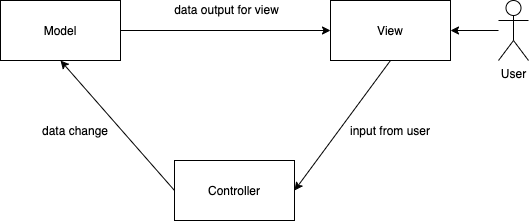
\includegraphics[width=1.00\textwidth]{mvc-diagram}		
		\caption{Komunikacja pomiędzy komponentami we wzorcu MVC }
\end{figure}

Zalety korzystania z wzorca MVC to lepsza przejrzystość kodu, skalowalność i utrzymanie. W
momencie wystąpienia błędu, może zostać obarczona odpowiedzialnością jedna z trzech części
systemu, więc optymalizuje to znacząco proces szukania miejsca, w którym dany błąd
występuje.  

\section{Wymagania funkcjonalne i niefunkcjonalne}
\paragraph{Wymagania funkcjonalne}
\begin{enumerate}
	\item Przegląd listy użytkowników
	\item Przegląd listy zadań 
	\item Tworzenie, edytowanie, usuwanie zadań
	\item Korzystanie z Tablicy Kanban w celu raportowania postępów w zadaniach
	\item Wyświetlanie Statystyk projektu w postaci wykresów
	\item Podstawowa autentykacja użytkownika
	\item wyświetlanie szczegółów związanych z danym zadaniem. Szczegółowe parametry zadania to:
	\begin{enumerate}[leftmargin=3em]
		\item nazwa,
		\item data do zakończenia zadania,
		\item użytkownik przypisany do zadania, 
		\item kolumna w której aktualnie znajduje się dane zadanie,
		\item opis zadania
		\item sekcja komentarzy
		\item nazwa użytkownika tworzącego zadanie
	\end{enumerate}
\end{enumerate}
\paragraph{Wymagania funkcjonalne dodatkowe dla administratora}

		\begin{enumerate} 
		\item tworzenie, aktywacja kont użytkowników, dostęp do większej ilości danych w porównaniu do użytkownika
		\item ustawienie czasu po jakim czyszczona jest historia czynności związanych z zadaniami 
		\item Konfiguracja tablicy:
	\begin{enumerate}[leftmargin=3em]
			\item określenie nazwy tablicy i kolumn
			\item określenie liczby kolumn, 
			\item wybranie domyślnej kolumny (na którą wprowadzane będą nowe zadania)
			\item wybranie końcowej kolumny (kolumna,która automatycznie zmienia status zadania na skończony), Opcjonalne
		\end{enumerate}

\end{enumerate}
\paragraph{Wymagania niefunkcjonalne}
\begin{enumerate}
	\item możliwość użytkowania systemu po godzinnym szkoleniu
	\item komunikacja z bazą dancyh nie dłuższa niż 200ms na każde zapytanie 
	\item aplikacja responsywna, aby nie było problemu wykonywać wszystkie założenia funkcjonalne na urządzeniu mobilnym
\end{enumerate}


\section{Diagram pakietów}





\section{Projekt bazy danych}

Sekcja ta w pełni skupiona jest na budowie bazy danych. Najpierw zdefiniowane zostały dane potrzebne do przechowywania.
Pierwszym rodzajem danych jest Tablica (tabela board), która przetrzymuje informacje o tablicy, z ilu  składa się kolumn, która kolumna jest kolumną domyslna, a która zamykającą zadania.
Kolejnym typem potrzebnym do przechowywania będzie wyżej wspomniana kolumna, która przechowuje status nazwę, kolejnosć wyswietlania na tablicy. Kolejnym typem jest Użytkownik, to jedna z najbardziej skomplikowanych tabel w całej bazie, ponieważ jest ona w relacji z zadaniami, które stworzył (mapowane poprzez pole ownedBy), w relacji z zadaniami do których jest aktualnie przypisany (pole assignedTo). Tabela z użytkownikami przetrzmuje informacje dotyczące korzystania z aplikacji i te  pozwalające autoryzować sesję po stronie klienta. Posiada również relacje z tabelą authority, która znowu odpowiedzialna jest za nadawnianie odpowiednich uprawnień do korzystania z aplikacji. Ostatnim z ważniejszych typów danych jest Zadanie i Komentarz. Zadanie jest to typ opisujący jak tylko może zadanie, przechowuje status w zależnosci od kolumny w której zadanie się znajduje, użytkowników powiązanych z utworzeniem zadania/ pracą nad zadaniem, a ostatnim typem będzie komentarz czyli tabela przetrzymująca komentarze odnoszące się do różnych zadań.

Jako serwer bazy danych wykorzystany został MySql serwer jako że jest to ....
W celu kontroli wersji projektu bazy danych do serwera podpięta jest biblioteka zwana Liquibase, która przechowuje wszystkie skrypty związane z tworzeniem bazy danych, modyfikacją tabel lub danych w formacie XML. Liquibase pomaga wprowadzać zmiany na istniejącej bazie danych przy zachowaniu poprzedniego stanu, zostawiając po udanej modyfikacji historię zmian. 

\section{Przypadki użycia}

W tym podrozdziale przedstawione zostały najważniejsze przypadki użycia aplikacji.


\begin{table}[h!]

\begin{tabular}{ |p{2cm}||p{13cm}|  }
	
	\hline
	\multicolumn{2}{|c|}{Rejestracja nowego użytkownika} \\
	\hline
	Aktorzy: &klient , serwer autoryzacyjny administrator\\
	\hline
	Warunki wstępne: & sesja klienta nie jest autoryzowana\\ 
	\hline
	Scenariusz: &
	\begin{enumerate}[leftmargin=0em]
		\item klient wchodzi na panel rejestracji za pomocą linka "Create Account" lub używając przycisku na nagłówku strony 
		
		\item po wypełnieniu przez klienta formularzu rejestracyjnego zachodzi proces walidacji danych

		\item  gdy walidacja przeszła pomyślnie: system wyświetla komunikat o sukcesie rejestracji i informuje,że potrzebna jest jeszcze aktywacja konta

	\begin{enumerate}[leftmargin=2em]
	 	\item  System zapisuje dane na bazie, hasło zostaje zakodowane.
	 		
	 		\item  System generuje losowy 8-cyfrowy klucz aktywacyjny dla użytkownika i wysyła na podany w formularzu e-mail link aktywacyjny.
	 		
	 		\item Klient  aktywuje konto za pomocą linka, który otrzymał na skrzynkę pocztową e-mail.
	\end{enumerate}
		
		\item  gdy walidacja zauważyła błędy w formularzu: wyświetla się komunikat błędu, zaznaczone zostają błędne pola
			\end{enumerate}
\\
	\hline

\end{tabular}

	\caption{Przypadek użycia - rejestracja nowego użytkownika}
\end{table}

\begin{table}[h!]
\begin{tabular}{ |p{2cm}||p{13cm}|  }
	
	\hline
	\multicolumn{2}{|c|}{Logowaniea} \\
	\hline
Aktorzy: &klient , serwer autoryzacyjny, system prezentujący\\
	\hline
Warunki wstępne: & sesja klienta nie jest autoryzowana, klient posiada aktywne konto\\
	\hline
	Scenariusz: &
	\begin{enumerate}
		\item klient wchodzi na panel logowania za pomocą linka "Log int" lub używając przycisku na nagłówku strony 
		\item klient wprowadza prawidłowe dane, nie zaznacza pola 'remember me'
		\begin{enumerate}
			\item system sprawdza czy istnieje użytkownik o podanych informacjach kwalifikujących
			\item system autoryzacyjny odnajduje w bazie użytkownika,
			\item system wysyła do systemu prezentującego wiadomość o poprawnym procesie weryfikacji, więc użytkownik zostaje przekierowany do widoku głównego po udanym logowaniu i przyznawane są prawa do przeglądania stron odpowiednich dla roli użytkownika, czyli ROLE\_ADMIN lub ROLE\_USER
		\end{enumerate}
		\item klient wprowadza prawidłowe dane,  zaznacza pole 'remember me'	
		\begin{enumerate}
			\item system autoryzacyjny odnajduje w bazie użytkownika,
			\item system autoryzacyjny tworzy 20-cyfrowy unikalny kod zwany tokenem i umieszcza go dla danego użytkownika
			\item system wysyła do systemu prezentującego wiadomość o poprawnym procesie weryfikacji, więc użytkownik zostaje przekierowany do widoku głównego po udanym logowaniu i przyznawane są prawa do przeglądania stron odpowiednich dla roli użytkownika, czyli ROLE\_ADMIN lub ROLE\_USER
		\end{enumerate}
		\item klient wprowadza złe dane
		\begin{enumerate}
			\item	system nie odnajduje użytkownika o podanych informacjach kwalifikujących , komunikuje się z systemem prezentującym o braku podanego użytkownika
			\item  system prezentujący wyświetla komunikat o prawdopodobnie źle wpisanym loginie lub haśle.
		\end{enumerate}
	\end{enumerate}
	\\
	\hline

\end{tabular}
	\caption{Przypadek użycia - Logowanie}
\end{table}


\begin{table}[h!]
\begin{tabular}{ |p{2cm}||p{13cm}|  }
	
	\hline
	\multicolumn{2}{|c|}{Dodawanie Zadania} \\
	\hline
Aktorzy: &użytkownik, serwer prezentujący, serwer obsługujący bazę danych\\
	\hline
Warunki wstępne: &sesja użytkownika jest autoryzowana i jest on na stronie "Board" lub "Task List"\\
	\hline
	Scenariusz: &

\begin{enumerate}
	\item Użytkownik przechodzi do panelu tworzenia nowego zadania po wciśnięciu przycisku "Create Task" zarówno na stronie "Board" jak i "Tasks List"
	\item pojawia się formularz z informacjami do podania na temat zadania, niektóre niezbędne do stworzenia zadania, niektóre opcjonalne
	\item po ukończeniu wypełniania formularza i kliknięciu przycisku "OK" system waliduje poprawność otrzymanych danych:
	\begin{enumerate}
		\item gdy dane odnośnie zadania zgadzają się, użytkownik przekierowywany jest na stronę, z której otworzył panel tworzenia zadania
		\item gdy dane odnośnie zadania nie zgadzają się, panel prezenetujący wyświetla pola z błędnymi informacjami
		\item użytkownik może poprawić dane i próbować stworzyć zadanie ponownie
	\end{enumerate}
\end{enumerate}\\
\hline
\end{tabular}
	\caption{Przypadek użycia - Dodawanie Zadania}
\end{table}

\begin{table}[h!]
		
	\begin{tabular}{ |p{2cm}||p{13cm}|  }
		
		\hline
		\multicolumn{2}{|c|}{Oglądanie szczegółów Zadania, edytowania zadania i usunięcie zadania} \\
		\hline
Aktorzy: &użytkownik, serwer prezentujący, serwer obsługujący bazę danych\\
		\hline
Warunki wstępne: & sesja użytkownika jest autoryzowana i jest on na stronie "Board" lub "Task List"\\
		\hline
		Scenariusz: &
		
		\begin{enumerate}


	\item Użytkownik przechodzi do panelu uaktualniania istniejącego zadania po wciśnięciu przycisku "Go To Task", który wyświetlany jest dla każdego zadania na jednej z kolumn  listy zadań w panelu "Tasks List" 
	\item Użytkownik może również przejść do panelu uaktualniania za pomocą kliknięcia w kontener wizualizujący zadanie na tablicy kanban w panelu "Board"
		\begin{enumerate}
		\item system prezentujący wyświetla wszystkie informacje na temat istniejącego zadania oraz trzy przyciski " Delete" "Edit" "Go Back"
		\begin{enumerate}
			\item użytkownik wciskając przycisk "Delete" pytany jest ponownie o potwierdzenie, za pomocą wyskakującego komunikatu
			\item po potwierdzeniu za pomocą przycisku "OK" system obsługujący dane usuwa  zadanie z bazy danych
			\item użytkownik przekierowywany jest spowrotem do wcześniejszego widoku
		\end{enumerate}
		\begin{enumerate}
			\item użytkownik używa przycisku Edit, przez co system prezentujący nadaje kontenerom prezentującym informacje funkcję formularza i pojawia się przycisk "Ok", przez co użytkownik może uaktualnić odpowiednie pola i zatwierdzić zmiany przyciskiem 'ok' i 
		\end{enumerate}
		\begin{enumerate}
			\item użytkownik po obejrzeniu informacji na temat zadania może za pomocą przycisku " go Back" wrócić do wcześniej odwiedzanego panelu
		\end{enumerate}
	\end{enumerate}
\end{enumerate}\\
\hline
\end{tabular}
\caption{Przypadek użycia - Oglądanie szczegółów Zadania, edytowania zadania i usunięcie zadania}
\end{table}

\begin{table}[h!]
	\begin{tabular}{|p{2cm}||p{13cm}|  }

\hline
\multicolumn{2}{|c|}{Przeglądanie listy zadań} \\
\hline
Aktorzy: &użytkownik, serwer prezentujący, serwer obsługujący bazę danych\\
\hline
Warunki wstępne:& sesja użytkownika jest autoryzowana i wyświetlony jest panel listy zadań "Tasks List"\\
\hline
Scenariusz: &
\begin{enumerate}
\item użytkownik jest na panelu "Tasks List"
\item wyświetlana jest przez system prezentujący  lista zadań na którym widoczne są najważniejsze informacje
\item system prezentujący otrzymuje listę ograniczoną parametrami z serwera obsługującego bazę danych
\item użytkownik klikając na nazwę kolumny jest w stanie sortować ją rosnąco lub malejąco
\item ostatnią kolumną jest przycisk "Go to Task", dzięki któremu możemy przejść do panelu danego taska
\end{enumerate}\\
\hline
	\end{tabular}
\caption{Przypadek użycia -Przeglądanie listy zadań}
\end{table}




\begin{table}[h!]
	\begin{tabular}{|p{2cm}||p{13cm}|  }
		
		\hline
		\multicolumn{2}{|c|}{Przeglądanie listy użytkowników} \\
		\hline
Aktorzy: &użytkownik, serwer prezentujący, serwer obsługujący bazę danych\\
		\hline
Warunki wstępne: &sesja użytkownika jest autoryzowana i wyświetlony jest panel listy użytkowników  "Users List", rolą użytkownika jest "ROLE\_USER" , czyli uprawnienia zwykłego użytkownika\\
		\hline
		Scenariusz: &
		\begin{enumerate}
			\item użytkownik jest na panelu "Users List"
		\item wyświetlana jest przez system prezentujący  lista zadań na którym widoczne są najważniejsze informacje
		\item system prezentujący otrzymuje listę ograniczoną parametrami z serwera obsługującego bazę danych
		\item użytkownik klikając na nazwę kolumny jest w stanie sortować ją rosnąco lub malejąco
		\item ostatnią kolumną jest przycisk "Go to Task", dzięki któremu możemy przejść do panelu danego taska
		\end{enumerate}\\
	\end{tabular}
	\caption{Przypadek użycia - Przeglądanie listy użytkowników}
\end{table}



\begin{table}[h!]
	\begin{tabular}{|p{2cm}||p{13cm}|  }
		


		\hline
		\multicolumn{2}{|c|}{Przeglądanie panelu ze statystykami} \\
		\hline
		Akotrzy: & użytkownik, serwer \\
		\hline
	   Warunki wstępne: & sesja użytkownika jest autoryzowana i wypełniona są tabele związane z historią \\
		\hline
		Scenariusz: &
		\begin{enumerate}
			\item użytkownik jest na panelu " Charts"
			\item wyświetlane są przez system prezentujący  informacje na temat projektu i 3 wykresy związane ogólnie ze statystykami projektu
			\item niżej znajdują się dwie listy do wyboru, lista użytkowników i zadań.
			\item użytkownik wybiera odpowiednich użytkowników na liście, aby wyświetlić wykresy związane z ich wynikami w ostatnich 6 miesiącach
			\item użytkwnik wybiera odpowiednie zadania na liście, po czym wyświetalne zostają wykresy dla każdego odznaczonego zadania pokazującego cykl życia zadania,
		\end{enumerate}\\
	\hline
	\end{tabular}
	\caption{Przypadek użycia - Przeglądanie panelu ze statystykami}
\end{table}


\begin{table}[h!]
	\begin{tabular}{|p{2cm}||p{13cm}|  }
		
		
		
		\hline
		\multicolumn{2}{|c|}{Aktualizowanie zadania za pomocą tablicy Kanban} \\
		\hline
		Akotrzy: & użytkownik, serwer \\
		\hline
		Warunki wstępne: & sesja użytkownika jest autoryzowana i na tablicy znajdują się różne zadania \\
		\hline
		Scenariusz: &
		\begin{enumerate}
			\item użytkownik jest na panelu "Board" widizi wszystkie kolumny i zadania w nich
			\item użytkownik za pomocą wydarzenia przyciśnij i upuść przeciąga zadanie z kolumny A do kolumny B
			\item system odpowiednio zapisuje dane wydarzenie, sprawdzając czy kolumna B nie jest równocześnie kolumną zamykającą zadania
			\item  po upuszczeniu na kolumnę B zadanie znajduje się na liście zadań dla kolumny B, serwer zapisuje wydarzenie zarówno w informacjach na temat kolumny i zadania, ale także wprowadza wydarzenie do specjalnej tabeli archiwizującej.
		\end{enumerate}\\
		\hline
	\end{tabular}
	\caption{Przypadek użycia - Aktualizowanie zadania za pomocą tablicy Kanban}
\end{table}


\begin{table}[h!]
	\begin{tabular}{|p{2cm}||p{13cm}|  }
		
		
		
		\hline
		\multicolumn{2}{|c|}{Konfiguracja tablicy} \\
		\hline
		Akotrzy: & administrator, serwer \\
		\hline
		Warunki wstępne: & sesja użytkownika jest autoryzowana jako administrator  \\
		\hline
		Scenariusz: &
		\begin{enumerate}
			\item użytkownik wchodzi na panelu "Manage Board" z poziomu nagłówka strony 
			\item system wyświetla formularz związany z informacjami tablicy, czyli nazwy i id kolumny która jest kolumną domyślną i kolumną zamykającą cykl zadania
			\item  użytkownik zmienia odpowiednie parametry, a końcowe informacje wysyła do serwera po zaakceptowaniu przyciskiem "Ok"
			\item serwer weryfikuje poprawność danych i aktualizuje potrzebne informacje
		\end{enumerate}\\
		\hline
	\end{tabular}
	\caption{Przypadek użycia - Konfiguracja tablicy}
\end{table}




	\cleardoublepage
	
	\chapter{Interfejs użytkownika}
wstawienie skrinów aplikacji zauważenie ciekawych mechanizmów html css cytat książka html css
\section{Widok Logowania}
\section{Widok Listy Zadań}
\section{Widok Admina}
\section{Widok Statystyk}
\section{Widok Tablicy}
\section{Widok Szczegółów Zadania}
	\cleardoublepage
	
	\chapter{Implementacja systemu}
\thispagestyle{chapterBeginStyle}
W tym rozdziale opisane zostały aspekty implementacyjne takie jak wzorzec architektoniczny aplikacji, narzędzia użyte do stworzenia aplikacji i ciekawe problemy napotkane podczas tworzenia serwisu.
\section{Implementacja  wzorca  MVC}
Opis implementacji wzorca projektowego MVC podzielony został na przedstawienie modelu, widoku i kontrolera.
\paragraph{Model}

Model reprezentowany jest przez model w bazie danych oraz przez serwisy na serwerze. 
Każda tabela posiada swój serwis. Jest to komponent, który odpowiedzialny jest za odpowiednie wprowadzanie i wyciąganie potrzebnych informacji z tabeli, którą reprezentują. Model został opisany wraz z przedstawieniem projektu bazy danych 
\paragraph{View - Widok}


Widok zaimplementowany jest przy pomocy szkieletu architektonicznego Angular korzystającego z HTML oraz TypeScript. Podstawowym obiektem w szkielecie jest komponent, na który składa się również skryptowy plik html i css lub scss. Komponent jest definicją jednego z wielu widoków w aplikacji, które Angular przedstawia na głównej stronie 
\paragraph{Controller - Kontroler}


Kontroler zaimplementowany jest głównie po stronie serwera, lecz komponenty odpowiedzialne za widok posiadają w sobie wstępne modyfikacje na danych otrzymanych od użytkownika takie jak przykładowo walidacja tych danych. Zaletą podejścia, aby funkcje kontrolera spełnianie były praktycznie po otrzymaniu jakichkolwiek danych jest to, że informacje, które przychodzą do serwera, aby przeszły przez główną logikę serwera są danymi nie podatnymi na błędy, więc serwer odpowiedzialny za logikę, nie będzie musiał skupiać się na odsyłaniu błędnych danych z powrotem do widoku, a o wiele częściej będzie otrzymywać już poprawne dane. Wadą takiego podejścia jest większe skomplikowanie w kodzie, ponieważ walidacja odbywa się wtedy zarówno na serwerze jak i po stronie klienta. Aplikacja odpowiedzialna za widoku musi również posiadać wiedzę na temat modelu bazy danych i poszczególne cechy różnych danych, aby odpowiednia logika mogła zostać zastosowana.


\section{Użyte technologie}
Projekt w pełni kompatybilny z systemem Windows 10 wykorzystuje z najważniejszych technologii:
\begin{itemize}
	\item Java 11
	\item Angular 11
	\item Bootstrap 4.6
	
\end{itemize}
W języku programowania Java taką pomocniczą technologią jest szkielet architektoniczny Spring. Posiada on dużo przeróżnych gałęzi i jest najpopularniejszym pomocniczym narzędziem dla języka Java. Aplikacja TaskManager korzysta z gałęzi Spring Boot, Spring Security oraz Spring Data JPA. 

\textit{Spring Security} zapewnia odpowiednie klasy wspomagające konfigurację autoryzacji i kontroli dostępu do zaimplementowanego serwera. \cite{SpringSecurity}   

\textit{Spring Data JPA} ułatwia dostęp do bazy danych udostępniając potrzebne metody wyciągające odpowiednie informacje z bazy danych.\cite{SpringData}  

\textit{Spring Boot} to gałąź, która pomaga uporać się ze wszystkimi możliwościami tego szkieletu i pomaga skonfigurować aplikację. 
W tym celu korzystając z narzędzia Spring Boot Initializer \cite{SpringInitializr} cały szkielet projektu został zainicjalizowany i dostępny do pobrania.
Kolejnym z ważnych narzędzi pomocniczych użytych podczas implementacji serwera jest \textit{ Maven}. Jest to narzędzie, które ułatwia zarządzanie projektem, ujednolica budowanie i kompilowanie zaawansowanego projektu napisanego w języku Java \cite{ApacheMavenProject}. 

\section{Narzędzia pomocnicze i środowisko programistyczne }
Program napisany został przy pomocy \textbf{Inteliij IDEA} . Jest to środowisko programistyczne, które w pełni wspomaga pisanie dużych projektów w języku Java. Możliwość debugowania kodu i pomocne wtyczki, które przykładowo pomagają utrzymać czystość kodu to ważny element podczas tworzenia aplikacji.
Kolejnym niezbędnym narzędziem jest \textbf{Postman }, który pomaga testować zapytania do serwerowego API. Aby zobaczyć, czy widok otrzymuje odpowiednie dane od serwera, wymagane jest przetestowanie zapytań, w tym celu zamiast wywoływać ich ręcznie w aplikacji, wykorzystujemy dany program, w którym przybieramy rolę klienta serwera i wysyłamy odpowiednie zapytania, oczekując prawidłowych odpowiedzi. \cite{Postman}
Cały projekt znajdował się podczas produkcji kodu w systemie kontroli wersji Git, w celu ułatwionego dostępu i możliwości powrotu do różnych wersji projektu.\cite{git}


\section{Opis ważniejszych  implementacji}

\subsection{Bezpieczeństwo aplikacji}
\subsubsection{konfiguracja}
Klasa \textit{SecurityConfiguration} przetrzymuje konfiguracje związane z odpowiednim dostępem w zależności od pozwoleń zalogowanego użytkownika. Tak jak widzimy na kawałku kodu ~\ref{httpconfig} prawie wszystkie ścieżki są udostępnione dla każdej roli poza ścieżkami \textit{api/admin/**} i \textit{management/**}, do których dostęp ma jedynie użytkownik z rolą administratora

\subsubsection{Autoryzacja i tworzenie konta}
Tworzenie konta użytkownika polega na wprowadzeniu potrzebnych informacji takich jak login, hasło i email. Po zaakceptowaniu danych przez serwer stworzona zostaje encja użytkownika nieaktywnego. Generowany zostaje klucz, który wysyłany jest w postaci linka na podaną wcześniej skrzynkę pocztową. Po wejściu w odpowiednią ścieżkę przez link z wiadomości użytkownik aktywuje konto i może się zalogować ~\ref{register}

\clearpage
\begin{lstlisting} [ caption= Uproszczona metoda określająca dostęp do podanych ścieżek, captionpos=b, label={httpconfig}]
	http
	.authorizeRequests()
	.antMatchers("/api/**").permitAll()
	.antMatchers("/api/admin/**").hasAuthority(AuthoritiesConstants.ADMIN)
	.antMatchers("/api/**").authenticated()
	.antMatchers("/management/**").hasAuthority(AuthoritiesConstants.ADMIN);
\end{lstlisting}


\begin{lstlisting} [ caption= Metoda rejestrująca użytkownika , captionpos=b, label={register}]
	public User registerUser(AdminUserDTO userDTO, String password) {
		
		User newUser = new User();
		String encryptedPassword = passwordEncoder.encode(password);
		newUser.setLogin(userDTO.getLogin().toLowerCase());
		// new user gets initially a generated password
		newUser.setPassword(encryptedPassword);
		newUser.setFirstName(userDTO.getFirstName());
		newUser.setLastName(userDTO.getLastName());
		if (userDTO.getEmail() != null) {
			newUser.setEmail(userDTO.getEmail().toLowerCase());
		}
		newUser.setImageUrl(userDTO.getImageUrl());
		newUser.setLangKey(userDTO.getLangKey());
		// new user is not active
		newUser.setActivated(false);
		// new user gets registration key
		newUser.setActivationKey(generateRandomAlphanumericString());
		Set<Authority> authorities = new HashSet<>();
		authorityRepository.findById(AuthoritiesConstants.USER)
		.ifPresent(authorities::add);
		newUser.setAuthorities(authorities);
		userRepository.save(newUser);
		log.debug("Created Information for User: {}", newUser);
		return newUser;
	}
\end{lstlisting}
\clearpage
\subsection{Tablica przeciągnij i upuść}
Główny widok aplikacji to tablica, na której użytkownik jest w stanie za pomocą wydarzenia przyciskiem myszy przeciągnij i upuść (z angielskiego drag and drop), aktualizować zadania do odpowiedniej kolumny. W tym celu użyty został moduł z Angulara o nazwie DragDropModule \cite{draganddrop}. Posiada on opisane dyrektywy o określonych funkcjach takich jak:
\begin{itemize}
	\item cdkDrag - nadaje elementom możliwość przeciągnięcia,
	\item cdkDropList - element ten określa listę elementów \textit{cdkDrop}, który odpowiednio je sortuje i jest w stanie wywołać wydarzenie wprowadzenia nowego elementu \textit{cdkDropListDropped},
	\item cdkDropListGroup - jako rodzic elementów \textit{cdkDropList} ma możliwość połączenia wszystkich elementów \textit{cdkDropList}, aby mogły one współdzielić wszystkie elementy  \textit{cdkDrop}, dzięki czemu możliwe jest  przeniesienie elementu \textit{cdkDrop}  z \textit{cdkDropList} A do \textit{cdkDropList} B
\end{itemize}
Na załączonym uproszczonym kodzie źródłowym ~\ref{board} kontener \textit{div tasks-container} zawiera wszystkie elementy, które przypisane mają do siebie zadania. Wydarzenie przeciągnięcia zadania na jedną z list wywołuje metodę \textit{drop}, która zapisuje identyfikatory odpowiednio zadania przeciąganego, kolumny z którego zadanie zostało przeciągnięte oraz kolumny, do której przeciągnięto dany element.


\begin{lstlisting} [ caption= Uproszczony skrypt odpowiedzialny za widok tablicy , captionpos=b, label={board}]
	<div class="board-columns" cdkDropListGroup>
	  <div class="board-column" *ngFor="let column of cards">
	    <div class="tasks-container"
	     cdkDropList
	     [cdkDropListData]="column.tasks"
	     (cdkDropListDropped)="drop($event)">	
	      <div class="task" id="{{task.id}}" 
                *ngFor="let task of column.tasks" 
                (click)="showTask(task)" 
                [cdkDragDisabled]="task.completed" cdkDrag>
                <span class="task-child" >{{task.name}}</span>
	      </div>
	    </div>
	  </div>
	</div>
\end{lstlisting}
\clearpage
\subsection{Rysowanie wykresów}
Ważnym elementem aplikacji jest widok statystyk przedstawianych w postaci wykresów. Do rysowania wykresów użyta została biblioteka Angular Bootstrap 4 Charts. Biblioteka udostępnia nam dyrektywę \textit{mdbChart},
która to po podaniu odpowiednich parametrów rysuje wykres na kanwie. \cite{MdbAngularBootstrap} Potrzebne parametry to:
\begin{itemize}
	\item chartType typ wykresu, podczas implementacji użyty został typ kołowy chartType = "pie" i liniowy chartType = "line"
	\item datasets to atrybut odpowiedzialny za dane przedstawione na wykresie. Jest to podpisana tytułem lista wartości.
	\item labels to lista nazewnictwa wartości osi poziomej x
	\item colors lista określająca kolory poszczególnych grup wartości
	\item options to lista szczegółowych opcji dostępnych dla wykresu
\end{itemize}
Kod źródłowy przedstawia inicjalizacje wykresu ~\ref{wykres}. Dane pobierane są z bazy danych z trzech nierelacyjnych tabel, które przetrzymują datę i użytkownika wykonującego akcje takie jak przeniesienie zadania z kolumny A do kolumny B, zakończenie zadania czy też przypisanie go do jakiegoś użytkownika. Na podstawie tych tabel inicjalizowana jest lista wartości. Na stronie \textit{statistics} znajdują się cztery typy wykresów:
\begin{itemize}
	\item kołowy wykres przedstawiający postęp w projekcie dzieląc zadania na zrobione, przypisane i nieprzypisane
	\item kołowy wykres, który przedstawia liczbę zadań dla każdej kolumny
	\item liniowy wykres, który dla wymienionego w liście do wybrania zadania pokazuje w ostatnich sześciu miesiącach liczbę przenosin na tablicy oraz liczbę przydzieleń do użytkowników
	\item liniowy wykres dla każdego użytkownika pokazujący liczbę przydzieleń dla ostatnich sześciu miesięcy i liczbę zadań zakończonych
\end{itemize}


\begin{lstlisting} [ caption= Inicjalizacja wykresu , captionpos=b, label={wykres}]
	<div style="display: block; width: 60%;">
	<canvas mdbChart
	[chartType]="chartType"
	[datasets]="chartDatasets"
	[labels]="chartLabels"
	[colors]="chartColors"
	[options]="chartOptions"
	[legend]="true"
	(chartHover)="chartHovered($event)"
	(chartClick)="chartClicked($event)">
	</canvas>
	</div>
\end{lstlisting}

	\cleardoublepage
	
	\chapter{Instalacja i wdrożenie}
\thispagestyle{chapterBeginStyle}
W tym rodziale przeprowadzone zostały instrukcje do uruchomienia aplikacji
\section{Uruchomienie serwera}
 Osoba zainteresowana, która chciałaby uruchomić daną aplikację lokalnie na swojej maszynie, musi liczyć się z tym, że rozbudowana aplikacja posiada wiele zależności z innymi programami i konfiguracji, dlatego serwer oraz baza danych zostały skonteneryzowane.  Konteneryzacja to wprowadzenie aplikacji ze wszystkimi zależnościami i wymaganymi do uruchomienia programami do wirtualnej jednostki zwanej kontenerem. Kontener to proces odizolowany od wszystkich innych procesów na maszynie hosta. Proces ten przeprowadzony został za pomocą programu \textit{Docker} \cite{docker}. 
 \paragraph{Instalacja programu Docker} 
 Platforma jest w pełni kompatybilna z systemem \textit{linux}, dla systemu \linebreak macOS i Windows docker udostępnia nakładkę pozwalającą korzystać z funkcji programu. Można pobrać go z oficjalnej strony :  \textit{\url{https://docs.docker.com/get-docker/}} 
 Po zainstalowaniu \textit{Dockera} w głównej gałęzi projektu \textit{./tmapp/}, gdzie znajduje się plik \textbf{docker-compose.yml}  wykonać w terminalu komendę:
 
 \begin{lstlisting}
docker-compose up --build -d
 \end{lstlisting}


Stworzone zostaną dwa kontenery, które przetrzymują serwer aplikacji i serwer bazy danych. Aby sprawdzić informacje na temat kontenerów należy wykonać komendę:
 
 \begin{lstlisting}
docker ps
\end{lstlisting}

Dzięki temu, że aplikacja została zkonteneryzowana, wystarczy pobrać \textit{dockera}, aby wywołać odpowiednie kontenery, które same doinstalują i zbudują projekt serwera. Aplikacja klienta nie została zdokeryzowana (inaczej konteneryzacja dzięki \textit{Docker}), ponieważ nie było to optymalne rozwiązanie. Framework \textit{Angular} wczystuje sporą liczbę plików przy budowaniu projektu przez co kontener ważyłby o wiele więcej. Podczas próby konteneryzacji trzech elementów, zauważony został zauważalny wzrost czasu załadowywania widoków na stronie oraz wydłużyła się komunikacja między serwerem.
\clearpage
\section{Uruchomienie klienta}
Kolejnym krokiem jest uruchomienie aplikacji klienta.
W tym celu potrzebujemy środowisko \textit{node.js}, aby zainstalować szkielet \textit{Angular}. W tym celu pobieramy ze strony: \textit{\url{https://nodejs.org/en/download/}} 
Podczas instalacji powinno kierować się domyślnymi konfiguracjami, które dodają odpowiednio program \textit{node} oraz \textit{npm}. Po instalacji można sprawdzić czy dane programy zostały odpowiednio zainstalowane za pomocą komend
 \begin{lstlisting}
	node --version
\end{lstlisting}
oraz
\begin{lstlisting}
	npm --version
\end{lstlisting}. Powinny zostać wyświetlone informacje na temat programu i jego zainstalowanej wersji. 

Kolejnym krokiem jest za pomocą programów wcześniej zainstalowanych instalacja szkieletu \textit{Angular}
Należy w wierszu poleceń wpisać następującą komendę:
\begin{lstlisting}
npm install -g @angular/cli
\end{lstlisting}
Dzięki wszystkim programom zainstalowanym powyższymi komendami możemy ostatecznie przejść do głównego folderu z aplikacją w wierszy poleceń: \begin{lstlisting}
	cd /path/to/rootfolder/tmapp/
\end{lstlisting}
Kiedy wiersz polecenia wskazuje na główny folder systemu, w którym znajduje się plik \textit{package.json}, zbudujemy projekt za pomocą komendy:

\begin{lstlisting}
npm install
\end{lstlisting}

Po pomyślnej inicjalizacji projektu i doinstalowaniu wszystkich potrzebnych paczek zewnętrznych powinien zostać wyświetlony komunikat o sukcesie.
Ostatnim krokiem zostało włączenie aplikacji za pomocą komendy:
\begin{lstlisting}
ng serve
\end{lstlisting}
Gdy dany proces włączania aplikacji przejdzie pomyślnie, strona \textit{http://localhost:9000} zostanie włączona automatycznie w domyślnej przeglądarce internetowej danej maszyny.






	\cleardoublepage
	
	\chapter{Podsumowanie}

\section{podsumowanie pracy}
\thispagestyle{chapterBeginStyle}

Celem niniejszej pracy inżynierskiej było stworzenie aplikacji internetowej wspomagającej zarządzanie zadaniami, w oparciu zastosowaniu metody Kanban.  Głównym zadaniem aplikacji było usprawnienie pracy własnej lub pracy w grupie, przy odpowiednim podziale zadań oraz ustalaniu priorytetów. Co ciekawe, aplikacja pozwala zorganizować codzienne obowiązki i efektywnie wykorzystać czas, ale również jest przydatna w przedsiębiorstwach przy organizowaniu i nadzorowaniu pracy zespołu. Zaproponowana aplikacja pozwala na rezygnację z notatek, wszystkie plany i zadania możemy zapisać w jednym miejscu, modyfikować w dowolnym czasie, potrzebujemy jedynie dostęp do urządzenia elektronicznego i Internetu. Popularność istniejących na rynku aplikacji do planowania dowodzi, że istnieje spora grupa użytkowników, która chętnie skorzysta z zaproponowanego rozwiązania. 

\section{Plany rozwoju aplikacji}
Po zapoznaniu się z opiniami pierwszych użytkowników ważnym kierunkiem rozwoju aplikacji jest uczytelnienie i poprawa interfejsu użytkownika. Po okresie próbnym korzystania z aplikacji przez użytkowników, należy przeprowadzić ankietę lub zapoznać się z opiniami użytkowników na forach. Dzięki analizie zdania użytkowników aplikacja stanie się bardziej intuicyjna.
Kolejnym, bardziej przyszłościowym kierunkiem byłaby synchronizacja z kontem Google lub Microsoft. Dzięki temu moglibyśmy rozszerzyć funkcjonalności o posiadanie kalendarzu z wyświetlonymi datami z zadaniami jak i informacje odnośnie grafiku pracowniczego. Moglibyśmy również mieć odnośniki przy poszczególnych użytkownikach do ich skrzynki pocztowej email przez co komunikacja stałaby się o wiele łatwiejsza.  Jest to oczywiście proces, w którym aplikacja utraci cechę prostej, zwartej aplikacji, ale niestety będzie zależała też od innych, zewnętrznych rozwiązań. Dany pomysł na rozbudowę aplikacji możemy kontynuować za pomocą rozbudowy informacji na temat użytkownika, przypięcie do aplikacji osobistego kanału smtp, aby użytkownicy dostawali przypisane do ich kont skrzynki pocztowe mogli komunikować się między sobą wewnętrznie za pomocą utworzonych służbowych kont. Kalendarz synchronizujący grafik pracowniczy z datami ukończenia poszczególnych zadań też jest funkcjonalnością, która może zostać wdrożona bez obecności zewnętrznych aplikacji.


	
	\cleardoublepage
	%%%%%%%%%%%%%%%%%%%%%%%%%%%%%%%%%%%%%%%%%%%%%%%%%%%%%%%%%%%%%%%%%%%%%%%%%%%%%%
	%%%%%%%%%%%%%%%%%%%%%%%%%%%%%%% BIBLIOGRAFIA %%%%%%%%%%%%%%%%%%%%%%%%%%%%%%%%%
	%%%%%%%%%%%%%%%%%%%%%%%%%%%%%%%%%%%%%%%%%%%%%%%%%%%%%%%%%%%%%%%%%%%%%%%%%%%%%%

	\pagestyle{bibliographyStyle}
	\bibliographystyle{plabbrv}
	\bibliography{literatura}
	\thispagestyle{chapterBeginStyle}
    \addcontentsline{toc}{chapter}{Bibliografia}

	\cleardoublepage

	\listoffigures
	\cleardoublepage
	\lstlistoflistings
	\cleardoublepage
	%%%%%%%%%%%%%%%%%%%%%%%%%%%%%%%%%%%%%%%%%%%%%%%%%%%%%%%%%%%%%%%%%%%%%%%%%%%%%%
	%%%%%%%%%%%%%%%%%%%%%%%%%%%%%%%%% DODATKI %%%%%%%%%%%%%%%%%%%%%%%%%%%%%%%%%%%%
	%%%%%%%%%%%%%%%%%%%%%%%%%%%%%%%%%%%%%%%%%%%%%%%%%%%%%%%%%%%%%%%%%%%%%%%%%%%%%%
	
	\appendix
	\pagestyle{appendixStyle}
	
	\chapter{Zawartość płyty CD}
\thispagestyle{chapterBeginStyle}
\label{plytaCD}

Płyta CD zawiera pracę pisemną w formacie \textbf{PDF} oraz katalog o nazwie \textit{tmapp}, który przechowuje tylko pliki źródłowe.
Pliki źródłowe serwera znajdują się w podkatalogu \textit{tmapp/src/main/java}, a pliki źródłowe klienta znajdują się w podkatalogu \textit{tmapp/src/main/webapp}
W katalogu głównym znajdują się również pliki konfiguracyjne odpowiedzialne za prawidłowe zbudowanie oraz uruchomienie aplikacji. 

	\cleardoublepage

\end{document}

